\RequirePackage{amsthm} %https://tex.stackexchange.com/questions/687324/unknown-theoremstyle-warning-with-springer-nature-template
\documentclass[sn-mathphys-num,iicol]{sn-jnl}

%\usepackage{sn-jnl.sty}
\usepackage{graphicx}%
\usepackage{multirow}%
\usepackage{amsmath,amssymb,amsfonts}%
\usepackage{amsthm}%
\usepackage{physics}
\usepackage{siunitx}
\usepackage{mathrsfs}%
\usepackage[title]{appendix}%
\usepackage{xcolor}%
\usepackage{textcomp}%
\usepackage{manyfoot}%
\usepackage{booktabs}%
\usepackage{algorithm}%
\usepackage{algorithmicx}%
\usepackage{algpseudocode}%
\usepackage{listings}%
\usepackage{newtxmath}%
\usepackage[tiny]{titlesec}%
\usepackage[ngerman]{babel}

\theoremstyle{thmstyleone}
\newtheorem{theorem}{Theorem}
\newtheorem{proposition}[theorem]{Proposition}

\theoremstyle{thmstyletwo}
\newtheorem{remark}{Remark}

\theoremstyle{thmstylethree}
\newtheorem{definition}{Definition}

\raggedbottom

\newcommand{\td}{\text{d}}

\titleformat{\subsection}{}{\thesubsection}{1em}{\itshape}

\begin{document}
        
\title[Title]{Das Magnetische Moment des Protons}
\author*[1]{\fnm{Jonas} \sur{Wortmann}}\email{s02jwort@uni-bonn.de}
\affil*[1]{Rheinische Friedrich--Wilhelms--Universität, Bonn}

\abstract{
Die Entdeckung des Protons durch \textsc{Rutherford} wird dargestellt und die physikalischen Größen des magnetischen Moments sowie des Magnetons werden erläutert.
Es wird das Protonenmoment in Bezug auf seine historische Bedeutung als erstes Indiz für die Substruktur des Protons erklärt.
Hierfür wird der experimentelle Aufbau von \textsc{Frisch} und \textsc{Stern} aus dem Jahr 1933 zur Bestimmung des Protonenmoments erklärt, die Auswertung dargestellt und das Ergebnis in Hinblick auf die damaligen Erwartungen diskutiert.
Im Anschluss wird ein Ausblick in aktuelle Forschungsthemen gegeben.
}

\maketitle

\section{Einleitung}
Das Protonenmoment ist eine wichtige physikalische Größe, sowohl im Kontext historischer Betrachtung, als auch vor dem Hintergrund der aktuellen Forschung.

Historisch führte das Protonenmoment zu Überlegungen über den Aufbau der Protonen.
Durch Messung des magnetischen Moments wurde erkannt, dass die damals gängige Theorie des Protons den experimentellen Ergebnissen nicht genügt.

In der aktuellen Forschung findet sich das Protonenmoment vor Allem im Vergleich mit dem Antiprotonenmoment, um Aussagen über die Charge--Parity--Time--Symmetrie (CTP--Symmetrie) und Materie--Antimaterie Asymmetrie zu treffen.
Ein wichtiger Anwendungsbereich in der Medizin ist die Magnetresonanztomographie (MRT), die es ermöglicht ohne schädliche Strahlung Bilder von Gewebe zu erzeugen.

\section{Die Entdeckung des Protons}
In einem Experiment im Jahre 1913 beschossen \textsc{Rutherford} und \textsc{Mardsen} ein Gasgemisch (Luft) mit $\alpha $--Teilchen, um den inneren Aufbau der Atome zu erforschen.

Die $\alpha $--Teilchen stammten aus einer radioaktiven Probe, deren Teilchenstrahl auf Luft gerichtet war.
Ein Zinksulfidschirm war um die Luft herum angebracht, welcher als Teilchendetektor diente.
Die Entfernung des Schirms von dem Gas war wesentlich größer als die Reichweite der $\alpha $--Strahlung, um zu vermeiden, das diese auf dem Schirm hätte detektiert werden können.

Das Ergebnis des Experiments zeigte, dass die $\alpha $--Teilchen an der Luft stießen und dabei Wasserstoffkerne aus dem Gas lösten, welche als Aufblitzen auf dem Schirm beobachtbar waren.

\textsc{Rutherford} wiederholte das Experiment mit Stickstoff.
Hierbei beobachtete er dasselbe Aufblitzen wie bei Luft, woraus er schlussfolgerte, dass Stickstoff aus Wasserstoffkernen bestehen muss.

Die Entdeckung des Protons wird einer Aussage um 1920 von \textsc{Rutherford} zugeschrieben, bei der er seine Beobachtungen aus dem Experiment verallgemeinerte.
Er behauptete, dass jedes Atom aus Wasserstoffkernen bestehen muss.
Zur Unterscheidung von ionisiertem Wasserstoff, nannte er diese Bestandteile Protonen.\cite{Rutherford_proton_discovery}\cite{Rutherford1919}

\section{Das magnetische Moment und das Magneton}
Die klassische Betrachtung des magnetischen Moments des Protons liefert die Stärke und Richtung eines magnetischen Dipols $\boldsymbol{m}~=~\tfrac{1}{2}\int\td ^3r\left[\boldsymbol{r} \times \boldsymbol{j} \left(\boldsymbol{r} \right)\right]$.
Betrachtet man einen Strom, der um eine Fläche kreist, so ergibt sich der Ausdruck $\boldsymbol{m} =I\cdot \boldsymbol{A} $.
Betrachtet man den Kreisstrom, erzeugt von einem geladenen Teilchen auf einer Kreisbahn, so ergibt sich mit $I=q/T$, mit der Periodendauer $T$, der Ladung $q$, und der Kreisfläche $|\boldsymbol{A} |~=~\pi r^2$ ein Moment von $|\boldsymbol{m} |~=~\tfrac{q}{T}\pi r^2$.
Der Bahndrehimpuls eines Teilchens auf einer Kreisbahn wird beschrieben durch $|\boldsymbol{l} |=\tfrac{2\pi }{T}mr^2$.
Bahndrehimpuls und magnetisches Moment lassen sich also miteinander verbinden zu $|\boldsymbol{\mu } |~:=~|\boldsymbol{m} |~=~\gamma |\boldsymbol{l} |~=~\tfrac{q}{2m}|\boldsymbol{l} |$.
Diese Größe wird auch als Magneton bezeichnet.

Die quantenmechanische Betrachtung des Magnetons liefert dann diskrete Werte, die proportional zu den Eigenwerten von $\hat{l}_z$ sind.
Wichtig für die folgende Diskussion sind das \textsc{Bohr}'sche Magneton für Elektronen mit der Drehimpulsquantenzahl $\ell=1$: $\mu _B=\tfrac{e\hbar }{2m_e}$; und das Kernmagneton, eine gängige Einheit in der Teilchenphysik, für Teilchen mit Spin $\tfrac{1}{2}$, $\ell=1$ und der Protonmasse: $\mu _N=\tfrac{e\hbar }{2m_p}$.

\section{Das Experiment von Otto Robert \textsc{Frisch} und Otto \textsc{Stern}}
\subsection{Motivation}
Die Motivation für dieses Experiment war die Untersuchung des Wasserstoffs mit dem Ziel der Bestimmung des Protonenmoments.
Darüber hinaus sollte auch eine allgemeine Apparatur zur Messung magnetischer Momente in der Größenordnung eines Kernmagnetons $\mu _N$ errichtet werden.
Die damals kürzliche Entdeckung des Ortho-- und Para--Wasserstoffmoleküls waren hierfür nützlich und wollten auch untersucht werden.

\subsection{Experimenteller Aufbau}
\noindent Der experimentelle Aufbau ist schematisch in Abb.\ (\ref{fig:experimenteller_aufbau_frisch_stern}) gezeigt.
Aus dem Ofen trat ein Molekülstrahl ($\text{H}_2$) aus, der mit Hilfe eines Abbildespaltes kollimiert wurde und in ein inhomogenes Magnetfeld eintrat.
In diesem Feld wurde der Strahl abgelenkt und die Intensität mit Hilfe des Auffängers (Manometer) gemessen.
Das Feld entstand durch Polschuhe, deren Querschnitt in Abb.\ (\ref{fig:experimenteller_aufbau_frisch_stern}) abgebildet ist.
Auf die exakte Anordnung und technische Details wird hier nicht weiter eingegangen.
Diese sind ausführlich in der Originalarbeit\cite{FrischStern1933} erklärt.
\begin{figure}[t]
        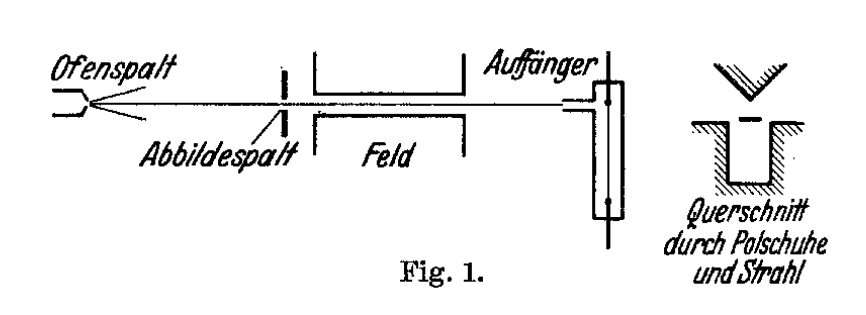
\includegraphics[width=.5\textwidth]{../vortrag/prosi_versuchsaufbau_mag_moment.png}
        \caption{Experimenteller Aufbau (schematisch); Gesamtlänge $\SI{30}{cm}$.\cite{FrischStern1933}}\label{fig:experimenteller_aufbau_frisch_stern}
\end{figure}

Im Folgenden werden die Anforderungen und Schwierigkeiten aufgeführt.
Der Strahl musste aufgrund der kleinen magnetischen Momente lang und schmal sein, damit die Abweichungen der Feldeinwirkung entsprechend groß und genaue Messungen möglich waren.
Der kleinste im Experiment verwendete Strahl hatte einen Durchmesser von circa $\SI{0.03}{mm}$.
Wichtig waren große Inhomogenitäten im Feld.
Diese lagen im Bereich von circa $\SI{22}{T/cm}$.
Für einen Strahl mit einem magnetischen Moment von einem Kernmagneton war dann eine Abweichung von $s~=~\SI{0.0044}{mm}$ zu erwarten.

Besondere Schwierigkeiten ergaben sich aus der Natur des Molekülstrahls ($\text{H}_2$).
Die Moleküle im Strahl waren \textsc{Maxwell}--verteilt, sie besaßen daher unterschiedliche Geschwindigkeiten und erfuhren unterschiedlich starke Ablenkungen.
Aus diesem Grund konnte die Ablenkung -- alleine verursacht durch das magnetische Moment -- nicht abgelesen werden, sondern musste aus der Intensitätsverteilung des Strahls berechnet werden.
Solch kleine Intensitäten konnten mit Hilfe sehr empfindlicher Manometer gemessen werden.
Technische Details sind in der Originalarbeit\cite{FrischStern1933} zu finden.

\subsection{Erwartungen}
Die Erwartung an das Experiment ergab für das Protonenmoment einen Wert von $\mu _p~=~1~\cdot~\mu _N~=~1~\cdot~\tfrac{e\hbar }{2m_p}$.
Diese Erwartung beruhte auf der Annahme, dass das Proton ein elementares \textsc{Dirac}--Teilchen ist; also punktförmig und ohne innere Struktur.
Diese Annahme lag in anbetracht des wissenschaftlichen Standes sehr nahe, da unter anderem das Elektron passend durch die \textsc{Dirac}'sche--Theorie beschrieben ist.

Der Wert des Protonenmoments sollte sich, nur aufgrund des Massenunterschieds, um einen Faktor von circa 1840 von dem des Elektrons unterscheiden.\cite{FrischStern1933}

\subsection{Durchführung \& Auswertung}
Das Gesamtmoment des $\text{H}_2$ ist eine Zusammensetzung aus dem Rotationsmoment und dem Kernmoment.
Das Kernmoment ist nicht exakt das Protonenmoment, da es sich hier um das $\text{H}_2$--Molekül handelt; das Protonenmoment konnte aber aus dem Kernmoment berechnet werden.

Die Beobachtung und Auswertung wurden an Ortho-- und Parawasserstoffmolekülen durchgeführt, da ihre magnetischen Eigenschaften hilfreich zur Bestimmung der einzelnen Momente waren.

Das $\text{H}_2$--Molekül hat, aufgrund des \textsc{Pauli}--Prinzips, zwei mögliche Spinanordnungen.
In Ortho--$\text{H}_2$ ist die Ausrichtung $\ket{\uparrow\uparrow}$ zu finden; in Para--$\text{H}_2$ $\ket{\uparrow\downarrow}$.
Dies bedeutet, dass Ortho--$\text{H}_2$ ein Kernmoment ungleich Null und Para--$\text{H}_2$ ein Kernmoment gleich Null hat.
Für beide Arten des Moleküls erwartete man daher unterschiedliche Aufspaltungsbilder.
In Abb.\ (\ref{fig:ortho_aufspaltung}) ist dies beispielhaft für Ortho--$\text{H}_2$ gezeigt. 
\begin{figure}[t]
        \centering
        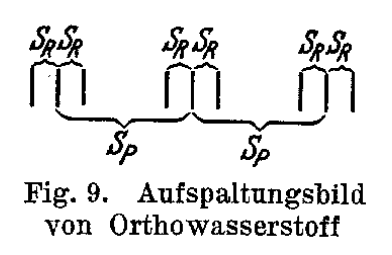
\includegraphics[width=.3\textwidth]{../vortrag/prosi_aufspaltungsbild_orthowasserstoff.png}
        \caption{Das Aufspaltungsbild von Ortho--$\text{H}_2$.\cite{FrischStern1933}} \label{fig:ortho_aufspaltung}
\end{figure}
Dabei beschreibt $S_R$ die Aufspaltung aufgrund des Rotationsmoments und $S_P$ die Aufspaltung aufgrund des Kernmoments.

Ziel dieser Auswertung war die Bestimmung des Kernmoments, um Rückschlüsse auf das Protonenmoment zu ziehen.
Dafür musste das Rotationsmoment von $\text{H}_2$ bestimmt werden, um dieses im Anschluss von dem Gesamtmoment zu subtrahieren.
Die Berechnung folgte aus der Intensitätsverteilung von Para--$\text{H}_2$ (zu sehen für gewöhnliches $\text{H}_2$ in Abb.\ (\ref{fig:graph})), da eine Bestimmung durch direkte Auswertung der Ablenkung des Strahls aufgrund der Messgenauigkeit nicht möglich war.
Para--$\text{H}_2$ wurde deshalb verwendet, weil sein Kernmoment Null ist und daher das Gesamtmoment nur aus dem Rotationsmoment besteht.
\begin{figure}[t]
        \centering
        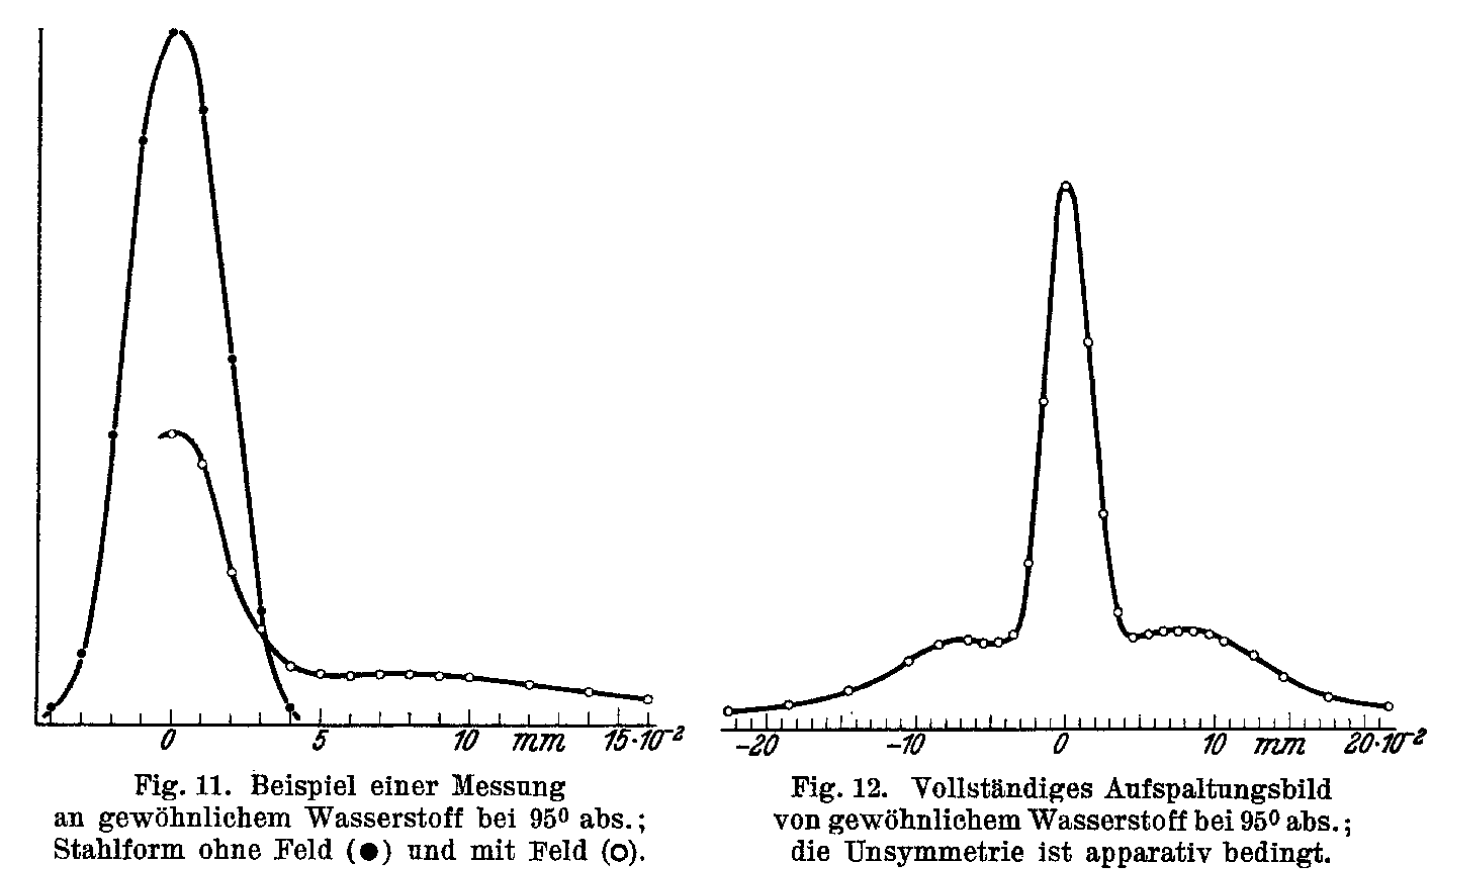
\includegraphics[width=.5\textwidth]{../vortrag/prosi_frisch_stern_auswertung_graph.png}
        \caption{Intensitätsverteilung des Molekülstrahls. Rechts ist eine Vergrößerung.\cite{FrischStern1933}} \label{fig:graph}
\end{figure}

Para--$\text{H}_2$ ist \textsc{Boltzmann}--verteilt, was bedeutet, dass $73\%$ der Moleküle die Rotationsquantenzahl $n=0$ und $27\%$ $n=2$ haben.
Für den Anteil mit $n=0$ ergab sich keine Ablenkung, was dem Peak der Intensitätsverteilung um die Ablenkung von $\SI{0}{mm}$ entspricht (s.\ Abb.\ \ref{fig:graph}).
Für den Anteil mit $n=2$ ergab sich eine Aufspaltung aufgrund der Aufhebung der Entartung.
Man erhielt jeweils Anteile der Intensitäten von $\tfrac{1}{5}$ für $m_n\in\left\{-2,-1,0,+1,+2\right\}$ die je ein abiträres Rotationsmoment (--quant) von $m_n\cdot \mu _R$ besaßen.
Es ergab sich also ein analoges Bild zu Abb.\ (\ref{fig:ortho_aufspaltung}) nur mit 5 anstatt 9 Intensitätsmaxima.

Dieses Rotationsmoment $\mu _R$ wurde wie folgt bestimmt.
Man berechnete eine erwartete Intensität für ein gewähltes $\mu _R$ und verglich diese mit der tatsächlich gemessenen Intensität.
Stimmen diese Intensitäten nicht überein, so wird $\mu _R$ weiter variiert.
Für ein ausgezeichnetes $\mu _R$, welches genau dem Rotationsmoment des Molekülstrahls entspricht, sind diese Intensitäten gleich.

Das Rotationsmoment von Para--$\text{H}_2$ ergab sich zu $\mu _R\lesssim \mu _N$.
Dieses Rotationsmoment ist auch der Wert für gewöhnliches $\text{H}_2$.
Misst man das Gesamtmoment über die selbe Methode so kann das Kernmoment von $\text{H}_2$ berechnet werden.\cite{FrischStern1933}

\subsection{Ergebnis}
Die im vorigen Abschnitt diskutierte Auswertung gab für das magnetische Moment des Protons einen Wert von $3\mu _N\leq \mu _p\leq 5\mu _N$.
Dieses Ergebnis war nicht mit der Erwartung von $\mu _P~=~\mu _N$ vereinbar \cite{FrischStern1933}.
Aus moderner Forschungsperspektive ist dieser Wert hingegen sehr gut zu erklären.
Das Proton ist kein elementares Punktteilchen, sondern aus Quarks zusammengesetzt $\left(u,u,d\right)$.
Das Protonenmoment berechnet sich also aus dem Moment der Quarks mit $\mu _p~=~\tfrac{3}{4}\mu _u~-~\tfrac{1}{3}\mu _d~\approx~ 2.792\mu _N$\cite{CODATA_proton_magneton}.

Obwohl dieses Ergebnis in der Originalarbeit nicht gedeutet wurde, ist es ein wichtiges Ereignis, bei dem die Struktur des Protons erstmals in Frage gestellt wurde.

\section{Die Substruktur des Protons}
Eine theoretische Analyse der Substruktur von Teilchen haben erstmals \textsc{Gell--Mann}\cite{Gellmann1964} und \textsc{Zweig}\cite{Zweig1964} 1964 unabhängig voneinander vorgenommen.

In \cite{Gellmann1964} stellt \textsc{Gell--Mann} ein Modell dar, indem Teilchen aus anderen Teilchen, namentlich \textit{Quarks}, aufgebaut werden können.
Es ergab sich, dass Baryonen aus einer ungeraden Anzahl an Quarks, also $\left(q,q,q\right)$, $\left(q,q,q,q,\overline{q}\right)$ etc.\ und Mesonen aus einer geraden Anzahl, also $\left(q,\overline{q}\right)$, $\left(q,q,\overline{q},\overline{q}\right)$ etc.\ aufgebaut werden können.
Er zeigte, dass der von ihm beschriebene \textit{Eightfold Way} zur Kategorisierung von Teilchen mit seinem Quark--Modell vereinbar ist.

Eine analoge, allerdings nicht auf dem \textit{Eightfold Way} beruhende Erklärung, wurde von \textsc{Zweig}\cite{Zweig1964} geliefert.
In seiner Ausarbeitung stellte er diese Elementarteilchen als Aces vor.

Diese Modelle wurden kurz nach ihrer Veröffentlichung am SLAC (Stanford Linear Accelerator Center) Experiment bestätigt.\cite{Bloom1969}
Bei Elektron -- Proton Streuung wurde der Formfaktor gemessen, welcher ergab, dass die Ladungsverteilung innerhalb des Protons punktförmig sein musste.
Dieses Ergebnis wurde in einer Ausarbeitung \cite{Bloom1969} von \textsc{Bloom}, et al.\ diskutiert und mit den von \textsc{Gell-Mann} beschriebenen Quarks identifiziert.

\section{Aktuelle Forschung}
In der modernen Forschung findet das Protonenmoment eine große Bedeutung, vor Allem im Hinblick auf die CPT--Symmetrie und Materie--Antimaterie Asymmetrie.
Anwendung findet das Protonenmoment in der Medizin, genauer in der MRT.

Am BASE im Cern\cite{BASE2017} wurde mit Hilfe von zwei \textsc{Penning}--Fallen das magnetische Moment des Antiprotons gemessen und mit dem magnetischen Moment des Protons verglichen.
Dabei konnten die Zyklotronfrequenz und \textsc{Larmor}-Präzession jeweils separat gemessen werden, um eine möglichst hohe Auflösung zu erreichen.
Es wurde nach Diskrepanzen gesucht, die auf mögliche Symmetriebrechungen hinweisen könnten.
Bisher sind die Momente beider Teilchen innerhalb der Fehlergrenzen kompatibel.

Die MRT beruht auf der Spin--Gitter und Spin--Spin Relaxation der Protonen in einem (organischen) Material.
Die Spins werden mit Hilfe eines homogenen Magnetfeldes ausgerichtet und anschließend durch Impulse magnetischer Wechselfelder ausgelenkt.
Diese Auslenkung ruft zwei Effekte hervor:
Die Spin--Gitter Relaxation, bei der sich die Protonenspins langsam entlang der homogenen Magnetfeldlinien ausrichten und dabei eine Änderung der Magnetisierung in der zum Feld orthogonalen Ebene gemessen werden kann;
und, die Spin--Spin Relaxation, bei der eine abnehmende Magnetisierung innerhalb der orthogonalen Ebene gemessen werden kann, die aufgrund der unterschiedlichen Präzessionsgeschwindigkeiten der Protonenspins zustande kommt.
Bei beiden Relaxationsprozessen wird eine Magnetisierung gemessen, die computergestützt in Bilder von Spindichten umgewandelt wird.
Diese geben Aufschlüsse über die Beschaffenheit der untersuchten Probe.

\bibliography{refs}

\end{document}
